\section{Introduction}

The contributions in this part of the thesis are focussed on the challenge of time domain Volterra series identification, and in particular, increasing the feasibility of parameter estimation for high series orders under general experimental conditions. In Chapter \ref{chap:4}, this issue was addressed from the perspective of computation time scaling, where the main optimization was reformulated into a method whose computational burden scales more favourably with series order.

There is another important factor affecting the feasibility of high order estimation, which is the sheer number of parameters required to be estimated in a time domain Volterra model. While the problem is particularly severe in multi-dimensional Volterra kernels, the desire to perform parameter reduction exists also in the linear impulse response case, from which inspiration can be drawn. In particular, orthonormal basis function modeling is a technique traditionally applied to linear systems \cite{Heuberger2005} that has also exhibited significant potential in the nonlinear domain \cite{Cheng2017}.

The use of orthonormal basis functions for linear system identification has been rigorously studied for several decades \cite{Heuberger2005}, \cite{Wahlberg1991}, \cite{Wahlberg1994}. The basic goal is to formulate a compact representation of a linear time-invariant (LTI) system by describing it as a weighted sum of rational orthonormal basis functions.  If the poles of the basis functions are chosen wisely, then only a small number of functions are required to sufficiently model the system behaviour.  Estimating the coefficients of the expansion is a linear-in-the-parameters problem, and the compact structure can produce lower variance estimates at the price of a small bias. Basis function representations are also possible in a Volterra series context \cite{Rugh1980}, however, placement of the basis function poles is more difficult to optimize in multi-dimensional kernels than in the linear case \cite{Campello2004}, \cite{Rosa2007}. 

This chapter makes a novel proposal to combine the parameter reduction technique of basis function modeling with the EM-based regularization method developed in Chapter \ref{chap:4}. By applying regularization directly on the more compact basis function model structure, the variance of model estimates can be dramatically reduced, along with their associated computation time. Theoretical justification is given for the use of regularization on higher-dimensional basis function expansions, and the EM method for hyperparameter tuning is modified to also iteratively optimize the basis function poles at each series order. A Monte Carlo simulation study is performed on example Volterra systems ranging from 2\textsuperscript{nd} to 5\textsuperscript{th} order, to compare the feasibility of high order parameter estimation using the proposed basis function method against the original regularized method in \cite{Birpoutsoukis2017}. 

\section{Orthonormal basis functions in identification}

The motivation for using orthonormal basis functions in linear identification stems directly from the shortcomings of FIR identification \cite{Heuberger2005}.  If we consider the impulse response, $h(\tau)$, generated by the rational transfer function, $G(z)$, we observe that if the poles of $G(z)$ are close to the unit circle, then $h(\tau)$ will tend to 0 very slowly with increasing $\tau$.  This implies that a large number of FIR parameters are required to accurately model the system. If we instead model the system $G(z)$ as a weighted sum of transfer functions $F_i(z)$ with impulse responses $f_i(\tau)$,
\begin{align}
\label{linearBF}
&G(z) = \sum_{i=1}^{\mathcal{B}} \alpha_i F_i(z) \\
\text{and } &h(\tau) = \sum_{i=1}^{\mathcal{B}} \alpha_i f_i(\tau),
\end{align}
with the poles of each $F_i(z)$ chosen carefully, the number of coefficients required to model $G(z)$ can be significantly reduced \cite{Heuberger2005}. 

When choosing a set of basis functions $F_i(z)$, it is desirable that the functions form a complete basis for the subspace of strictly proper, real, rational transfer functions. One class of basis functions which satisfy this criterion are the Takenaka-Malmquist functions \cite{Akcay1998}. The functions are constructed from a sequence of all-pass filters, whose poles, $a_i$, lie within the unit disc and satisfy the completeness condition, $$\sum_{i=1}^{\infty}(1-|a_i|)=\infty.$$ Their general form \cite{Heuberger2005} can be written as 
\begin{equation}
\begin{split}
\label{tak-malm}
F_i(z) &= \frac{\sqrt{1-|a_i|^2}}{z-a_i} \prod_{j=1}^{i-1} \frac{1-\bar{a}_jz}{z-a_j} \\
& = \frac{\sqrt{1-|a_i|^2}}{z-a_i} \prod_{j=1}^{i-1} G_j(z).
\end{split}
\end{equation}

The so-called Generalized Orthonormal Basis Functions (GOBFs) are obtained in the case where $G_j(z) = \bar{G}(z) \; \; \forall j$.  The McMillan degree of $\bar{G}(z)$ can also be made greater than 1, by taking a linear combination of the complex functions generated in (\ref{tak-malm}) \cite{Ninness1997}.  It follows that the total number of generating poles required to define a GOBF sequence is equal to the McMillan degree of $\bar{G}(z)$, which we will denote $d_G$. In the following sections we will examine more closely the case of $d_G =1$ and $d_G = 2$.

\subsection{Laguerre basis functions}
\label{sec:LBFdef}

Laguerre Basis Functions (LBFs) are a subset of the GOBFs which are parameterized by a single, real pole, such that $d_G$ = 1 for the all-pass filter $\bar{G}(z)$. This results in basis functions of the form
\begin{equation}
\label{LBFdef}
F_i(z) = \frac{\sqrt{1-|a|^2}}{z-a} \bigg( \frac{1-a z}{z-a} \bigg) ^{i-1}, \; \; \; a \in (-1,1).
\end{equation}
While the Laguerre functions are easy to construct with a simple structure, one distinct disadvantage is that the functions cannot be constructed using complex poles. As a consequence, a larger number of expansion coefficients are required to accurately model oscillatory systems \cite{Wahlberg1991}.  

\subsection{Kautz basis functions}
\label{sec:KBFdef}

In the case where $d_G = 2$, we can obtain the 2-parameter Kautz Basis Functions (KBFs)~\cite{Wahlberg1994}.  For these functions, the opportunity exists to incorporate a pair of complex poles into the generating all-pass filter in order to better model oscillatory responses.  In much the same way that the Laguerre functions were parameterized by a single real pole in (\ref{LBFdef}), the Kautz functions can be parameterized by two complex conjugate poles,  $[x+iy , x-iy]$. The problem with this parameterization is that the allowable ranges for $x$ and $y$ are interdependent, since $(x^2 + y^2) <1$ is required for stability of $\bar{G}(z)$ \cite{Heuberger2005}.  A more practical parameterization defines two new parameters,
$$a = \frac{2x}{1+x^2+y^2}, \; b = -(x^2+y^2),$$
such that the 2-parameter Kautz functions can be expressed in the form,
\begin{equation}
\begin{split}
\label{KBFdef}
&F_{2i-1}(z) = \frac{\sqrt{1-b^2}(z-a)}{z^2+a(b-1)z-b} \bigg( \frac{-b z^2 + a(b-1)z + 1}{z^2 + a(b-1)z - b} \bigg)^{i-1}, \\
&F_{2i}(z) = \frac{\sqrt{(1-b^2)(1-a^2)}}{z^2+a(b-1)z-b} \bigg( \frac{-b z^2 + a(b-1)z + 1}{z^2 + a(b-1)z - b} \bigg)^{i-1},
\end{split}
\end{equation}
where $a,b \in (-1,1)$. 

\section{Basis function expansions of Volterra models}

Using orthonormal basis functions in a Volterra series model is a concept referred to as the Volterra/Wiener approach \cite{Rugh1980}. In the same way that an impulse response, $h(\tau)$, can be approximated by a sum of basis responses in (\ref{linearBF}), higher-dimensional Volterra kernels can also be approximated using a sum of basis functions.  For a kernel, $h_m(\tau_1,\hdots,\tau_m)$, the basis function expansion can be expressed as
\begin{equation}
\label{OBF2Kernel}
h_m(\tau_1,\hdots,\tau_m) = \sum_{i_1=1}^{\mathcal{B}_m} \hdots \sum_{i_m=1}^{\mathcal{B}_m} \alpha_m(i_1,\hdots,i_m) \prod_{j=1}^{m} f_{m,i_j}(\tau_j), \; \; \; \; m = 1, \hdots, M,
\end{equation}
where $f_{m,l}(\tau)$ is the impulse response corresponding to the $l$\textsuperscript{th} basis function of the kernel $h_m$, $\mathcal{B}_m$ is the number of basis functions in the expansion, and $\alpha_m(\cdot)$ is the set of expansion coefficients. The time domain Volterra series model (\ref{eq:VolterraConvolutionDefn}) can be combined with (\ref{OBF2Kernel}) to restructure the model, i.e.
\begin{equation}
\begin{split}
\label{OBFvolterra}
y^0(t) &= \alpha_0 + \sum_{m=1}^{M} y_m(t), \\
y_m(t) &= \sum_{i_1=1}^{\mathcal{B}_m} \hdots \sum_{i_m=1}^{\mathcal{B}_m} \alpha_m(i_1,\hdots,i_m) \prod_{j=1}^{m} u^f_{m,i_j}(t)
\end{split}
\end{equation}
where $\alpha_0 = h_0$ from (\ref{eq:VolterraTimeDomainOutput}), and $u^f_{m,l}$ is the input, $u$, filtered by the $l$\textsuperscript{th} basis function of the $m$\textsuperscript{th} kernel's basis. Note the similarity in structure between the models in (\ref{eq:VolterraConvolutionDefn}) and (\ref{OBFvolterra}), which motivates the treatment of the expansion coefficient sets $\alpha_m$ as \emph{basis function kernels} in the domains of their corresponding bases. Taking this view, $\mathcal{B}_m$ is analogous to memory length, and the assumption of symmetry, as discussed in Chapter \ref{sec:VolterraProperties}, is equally valid with the same consequences for parameter estimation. The basis function kernels can be much more compact than their time-domain counterparts, provided that the bases are carefully designed \cite{Campello2004},\cite{Rosa2007}. Figure \ref{fig:CompactBFkernel} shows an example 2\textsuperscript{nd} order kernel in the time domain (left) and using a well parameterized LBF expansion (right).

\begin{figure}[h]
\centering
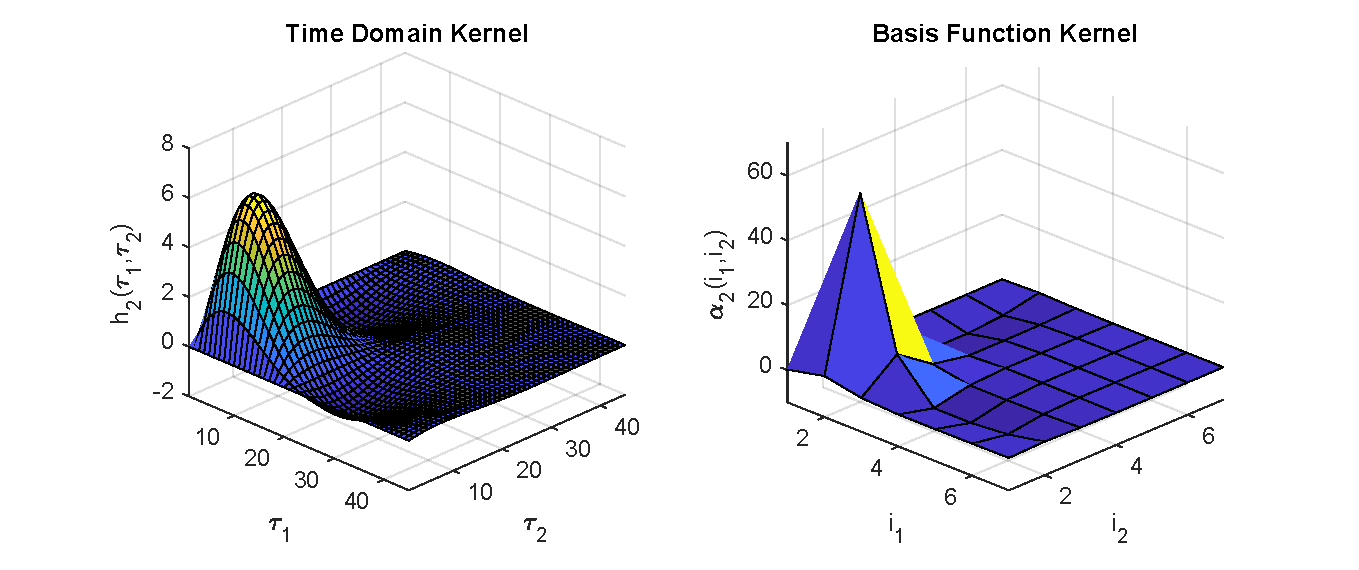
\includegraphics[width = 0.98\textwidth]{Chapter5_RegBFs/TDvsBFkernels3.pdf}
\caption{A well parameterized LBF kernel (right) is typically far more compact than its equivalent time domain kernel (left)}
\label{fig:CompactBFkernel}
\end{figure}

A linear regression formulation for the estimation of the $\alpha_m$ kernels is possible using the same framework described in Chapter \ref{sec:RegVolterraTD}. Based on Assumption \ref{ass:ReLSmodelstructure}, a regression model for the basis function expanded series (\ref{OBFvolterra}) can be given as
\begin{equation}
Y = \Phi_f^T \alpha + E,
\label{eq:RegressionStructure_OBFseries}
\end{equation}
where the regressor, $\Phi_{f}$, now contains appropriate \emph{filtered} input products. The parameter vector is still constructed as if the expansion coefficients $\alpha_m$ were standard Volterra kernels, i.e. $\alpha = [\alpha_0, {\alpha^{\mathcal{V}}_1}^T, \hdots , {\alpha^{\mathcal{V}}_M}^T]^T$, where $\alpha^{\mathcal{V}}_m$ denotes a vector of \emph{unique} $m$\textsuperscript{th} order expansion coefficients.

Naturally a least squares estimate of the basis function kernels is possible, provided that there is enough input/output data available, which is analytically computed using
\begin{equation}
\hat{\alpha}_{LS} = ( \Phi_{f}  \Phi_{f}^T)^{-1} \Phi_{f} Y.
\label{LSbf}
\end{equation}

So far we have assumed that a set of appropriate basis functions exist for each nonlinear order $m$. In reality, these basis functions must be chosen by the user, and ideally the functions for a kernel $h_m$ should reflect the system dynamics present in that kernel. The problem of selecting optimal basis functions for Volterra kernel expansion was considered in \cite{Campello2004} for the case of LBFs, and in \cite{Rosa2007} for the case of KBFs. Optimality here is defined by the minimization of error introduced from truncation of the LBF/KBF expansions to a finite length, $\mathcal{B}_m$. That is to say that an optimal basis will allow the most compact basis function kernel. 

\subsection{Optimal selection of Laguerre poles}
\label{sec:OptimalLBFpole}

We will consider a Volterra kernel $h_m$ of order $m$, which can be expressed as a Laguerre basis function expansion using (\ref{LBFdef}) and (\ref{OBF2Kernel}), parameterized by the pole $a  = a_m$.  It can be shown that minimizing the cost function, 
\begin{equation}
\label{LBFcost}
J_m(a_m) = \sum_{i_1}^{\infty} \hdots \sum_{i_m}^{\infty} (i_1 + \hdots + i_m) \alpha_m^2(i_1, \hdots , i_m),
\end{equation}
with respect to $a_m$ will also minimize the upper bound on the squared norm of the truncation error \cite{Campello2004}. Furthermore, there is a strict global solution to (\ref{LBFcost}) which can be obtained solely from the time-domain kernel.  The optimal pole can thus be calculated from $h_m$ \cite{Campello2004}, i.e.
\begin{equation}
a_m = \frac{2Q_{1,m}-1-Q_{2,m}}{2Q_{1,m}-1+\sqrt{4Q_{1,m}Q_{2,m}-Q_{2,m}^2-2Q_{2,m}}},
\end{equation}
where 
$$Q_{j,m}= \frac{1}{m} \sum_{l=1}^{m} S_{j,l},$$
$$S_{1,l} = \frac{1}{\| h_m \|^2} \sum_{\tau_1=0}^{\infty} \hdots \sum_{\tau_m=0}^{\infty} \tau_l h_m^2(\tau_1, \hdots, \tau_m),$$
$$S_{2,l} = \frac{1}{\| h_m \|^2} \sum_{\tau_1=0}^{\infty} \hdots \sum_{\tau_m=0}^{\infty} \tau_l [\Delta_l h_m(\tau_1, \hdots, \tau_m)]^2,$$
and the operators $\| \cdot \|^2$ and $\Delta_l$ are defined by
$$ \| h_m \|^2 = \sum_{\tau_1=0}^{\infty} \hdots \sum_{\tau_m=0}^{\infty} h_m^2(\tau_1, \hdots, \tau_m),$$
$$ \Delta_l  h_m = h_m(\tau_1, \hdots, \tau_l + 1, \hdots, \tau_m) - h_m(\tau_1, \hdots, \tau_l, \hdots, \tau_m).$$ 

\subsection{Optimal selection of Kautz poles}
\label{sec:OptimalKBFpoles}

For the 2-parameter Kautz case, we consider again the Volterra kernel $h_m$, expanded now using the Kautz functions defined in (\ref{KBFdef}). Unlike the Laguerre case, no analytic solution exists in the literature to find optimal Kautz parameterizations. However, sub-optimal estimates can be obtained by fixing $a = a_m$, as this provides an analytic solution \cite{Rosa2007} for optimizing $b = b_m$ at the given $a_m$ value. Combining this analytic, sub-optimal method with an exhaustive search through the space of valid $a_m$ values will then reveal the global optimum.

It can be shown \cite{Rosa2007} that the upper bound on truncation error resulting from expansion into Kautz functions is minimized by minimizing the cost function,
\begin{equation}
\label{KBFcost}
L_m(a_m,b_m) = \frac{q_2 b_m^2 - 2 q_1 b_m + q_3}{1-b_m^2},
\end{equation}
where the scalars $q_1, q_2, q_3$ are given by
\begin{align*}
&q_1 = \mu_1(g_{even}) + \mu_1(g_{odd}),\\
&q_2 = \mu_2(g_{even}) + \mu_2(g_{odd}),\\
&q_3 = q_2 + m \cdot \mu_3(g_{even}) + m \cdot \mu_3(g_{odd}).
\end{align*}
The moments $\mu_j$ are defined as,
\begin{align*}
\mu_1(g) &= \sum_{j=1}^{m} \Bigg[  \sum_{k_1=0}^{\infty} \hdots \sum_{k_j=0}^{\infty} \hdots \sum_{k_m=0}^{\infty} k_j \cdot g(k_1,\hdots,k_j,\hdots,k_m) \cdot g(k_1,\hdots,k_j-1,\hdots,k_m) \Bigg], \\
\mu_2(g) &= \sum_{j=1}^{m} \Bigg[  \sum_{k_1=0}^{\infty} \hdots \sum_{k_j=0}^{\infty} \hdots \sum_{k_m=0}^{\infty} k_j \cdot g^2(k_1,\hdots,k_m),\\
\mu_3(g) &= \sum_{k_1=0}^{\infty} \hdots \sum_{k_m=0}^{\infty} g^2(k_1,\hdots,k_m),
\end{align*}
and the functions $g_{even}$ and $g_{odd}$ are functions on the time domain kernel:
\begin{align*}
g_{even}(k_1, \hdots, k_m) &= \sum_{\tau_1=0}^{\infty} \hdots \sum_{\tau_m=0}^{\infty} h_m(\tau_1, \hdots, \tau_m) \cdot \prod_{j=1}^{m} \hat{f}_{2k_j+2}(\tau_j),\\
g_{odd}(k_1, \hdots, k_m) &= \sum_{\tau_1=0}^{\infty} \hdots \sum_{\tau_m=0}^{\infty} h_m(\tau_1, \hdots, \tau_m) \cdot \prod_{j=1}^{m} \hat{f}_{2k_j+1}(\tau_j),
\end{align*}
where $\hat{f}_{(\cdot)}$ are the Kautz function impulse responses with $b_m=0$. 

For a fixed value of $a_m$, (\ref{KBFcost}) is convex, and minimized by a specific selection of $b_m$~\cite{Rosa2007}, given by 
\begin{align*}
&b_m^* = 
\begin{cases}
\zeta - \sqrt{\zeta^2-1} &\text{if } \zeta>1, \\
\zeta + \sqrt{\zeta^2-1} &\text{if } \zeta<-1,
\end{cases} \\
\text{where } & \zeta = (q_2 + q_3)/2q_1
\end{align*}
Thus, by searching through a discretized space of $a_m \in (-1,1)$, we can analytically compute the optimal $b_m^*$ for each $a_m$, and the corresponding cost, $L_m(a_m,b_m^*)$. Once the discretized $a_m$-space has been searched, the parameter set which produced a globally minimum $L_m$ is the optimal choice for expansion of $h_m$. 

\section{Regularized identification of basis function kernels}
\label{RegBFs_Chap5}

The parallels between time domain and basis function Volterra models have motivated the treatment of expansion coefficients as \emph{basis function kernels} in the domains of their bases.  A natural progression then is to consider applying regularization to these new kernels in the same way that it was applied to time domain kernels, i.e. by imposing smoothness and decay along the hypersurfaces generated by the basis function expansions.

To this end, one can define a typical quadratically regularized estimator, 
\begin{align}
\label{ReBF}
\hat{\alpha}_{ReLS} &= \text{arg } \underset{\alpha}{\text{min}} \|Y - \Phi_{f}^T \alpha \|^2_2 + \sigma^2 \alpha^T P^{-1} \alpha \\
&= (P \Phi_f \Phi_f^T + \sigma^2 I)^{-1} P \Phi_f Y.
\label{eq:ReBFanalytic}
\end{align}  
As in Chapter \ref{sec:RegVolterraTD}, the penalty matrix $P$ can be constructed block diagonally using Bayesian prior covariances, with the following assumption. 
\begin{assum}
Every vector of expansion coefficients, $\alpha_m^\mathcal{V}$, is a zero mean Gaussian process: 
\begin{equation}
\alpha_m^\mathcal{V} \sim \mathcal{N}(0,P_m) \; \; \; m = 1, \hdots, M.
\end{equation}
Furthermore, all pairs of coefficient vectors, $\alpha_i^\mathcal{V}$ and $\alpha_j^\mathcal{V}$, are independent for $i \neq j$.

The constant offset is also Gaussian, i.e. $\alpha_0 \sim \mathcal{N}(0,P_0)$, and independent of the other processes.
\end{assum}

If we simply frame the basis function kernels as Volterra kernels in a different domain, then the prior covariance for each kernel can be formed via an identical procedure to the time domain case in (\ref{KernelPenalty}), (\ref{TCext})/(\ref{DCext}), and (\ref{FinalPenalty}). Furthermore, the hyperparameters may be tuned using the same EM-based optimization derived in Chapter \ref{chap:4} (Algorithm \ref{alg:EMtuning}). It should be noted, however, that for estimation using basis functions there is an added complication of choosing poles to generate the basis functions at each nonlinear order. These poles can be treated as additional hyperparameters requiring optimization, which requires some modifications to the EM tuning approach.  

\subsection{Theoretical justification}

To impose the same covariance structures on expansion coefficients that have been used on standard Volterra kernel parameters, there must be justification that the basis function kernels will in fact exhibit the same smooth, decaying behaviour. 

For linear FIR models, the concept of regularized basis function estimation has already been explored in \cite{Chen2015}, where the TC covariance structure was applied in regularized estimation of Laguerre coefficients. The approach was shown, in \cite{Darwish2018}, to be equivalent to applying a basis-function-based covariance structure directly on the time-domain FIR parameters. In the linear case, the justification for such an approach is trivial when using Laguerre or Kautz functions. In these cases, the set of expansion coefficients for a (rational) linear system are seen to be the impulse response of the system under a given transformation, where the transformation maps stable poles to other stable poles \cite{Heuberger2005}, \cite{Wahlberg1994}. This implies that the expansion coefficients are also free to be interpreted as a stable impulse response, with all the familiar smoothness and decay properties.   

For higher-dimensional Volterra kernels the linear justification is not applicable, because the definition of stability is more complex (see Chapter \ref{sec:VolterraProperties}), and the notion of poles in some rational linear filter may not exist for an arbitrary nonlinear system. In order to solve this issue, a Bayesian approach is proposed here to show that basis function kernels decay to zero in all causal directions of the hypersurface, so long as their time domain counterparts are well behaved. The approach will be demonstrated for the case of Laguerre basis functions.

\begin{thm}
\label{thm:DecayingLBFs}
If $h_m(\tau_1, \hdots, \tau_m)$ is an $m$\textsuperscript{th} order, zero mean Gaussian Volterra kernel with finite covariance, then any valid Laguerre basis function expansion of the kernel, $\alpha(i_1, \hdots, i_m)$, will decay to 0 in all causal directions.
\end{thm}

\begin{proof*}
Let $i_1 = x_1 s, \hdots, i_m=x_m s$, where $x_1, \hdots, x_m \geq 0$ and $s \to \infty$ is the limit of interest, i.e. we consider the limiting behaviour in some causal direction. 

The infinite basis function expansion is given by
\begin{align}
\alpha(i_1, \hdots, i_m) = \alpha(x_1 s, \hdots, x_m s) = \sum_{\tau_1=0}^{\infty} \hdots \sum_{\tau_m=0}^{\infty} h_m(\tau_1, \hdots, \tau_m) \prod_{j=1}^{m} f_{x_j s}(\tau_j)
\end{align}
where $f_{x_j s}$ is the impulse response for the $x_j s = i_j$\textsuperscript{th} Laguerre function. 

The mean of the expansion coefficients is trivially zero, since $h_m$ is a zero mean process.
The variance of the coefficients is given by
\begin{align}
\label{eq:AlphaVariance}
\Var[\alpha(x_1 s, \hdots, x_m s)] &= \sum_{\tau_1=0}^{\infty} \hdots \sum_{\tau_m=0}^{\infty} \sum_{q_1=0}^{\infty} \hdots \sum_{q_m=0}^{\infty} \nonumber \\ 
&\Cov[h_m(\tau_1, \hdots, \tau_m),h_m(q_1, \hdots, q_m)] \cdot \prod_{j=1}^{m} f_{x_j s}(\tau_j) f_{x_j s}(q_j). 
\end{align}
The Laguerre filters (\ref{LBFdef}) can be rewritten as
\begin{equation}
\label{eq:LongDivResult}
F_i(z)=\frac{0z^i + \sum_{k=0}^{i-1} p_{k,1}(i) a^k z^k}{z^i + \sum_{k=0}^{i-1} p_{k,2}(i) a^{i-k} z^k}, \; \; a \in (-1,1) \setminus \{0\},
\end{equation}
where $p_{m,n}$ are arbitrary polynomials in $i$ resulting from the binomial expansion.
Performing the division in (\ref{eq:LongDivResult}) gives the form for the first $i$ values of $f_i(\tau)$ (See Appendix \ref{append:LongDivision} for the division):
\begin{align*}
f_i(\tau) &= p_{l,j}(i)\cdot a^{i-\tau} \; \; \text{for} \; 0 \leq \tau<i , \; l,j \in \mathbb{Z}^+ \\
&\implies \lim_{i \to \infty} f_i(\tau) = 0\; \; \; \forall \tau \in \mathbb{Z}^+ 
\end{align*}
Hence $s \to \infty$ causes all $ f_{x_j s}(\tau_j), f_{x_j s}(q_j)$ to go to $0$ in (\ref{eq:AlphaVariance}), and since all kernel covariances are finite,
\begin{align*}
&\lim_{s \to \infty} \Var[\alpha(x_1 s, \hdots, x_m s)] = 0 
\end{align*} \qed
\end{proof*}

\begin{rem}
The smoothness of basis function kernels is not addressed in Theorem \ref{thm:DecayingLBFs}, despite being imposed by most common covariance structures. However, if we use the same Bayesian approach on the first order case as an example, the correlation between two expansion coefficients separated by $\epsilon \in \mathbb{Z}^+$ is given by:
$$\textbf{E}\{ \alpha(i) \alpha(i+\epsilon) \} = \sum_{\tau = 0}^{\infty} \sum_{\tau' = 0}^{\infty} \textbf{E}\{h(\tau)h(\tau')\} f_i(\tau) f_{i+\epsilon}(\tau'),$$
which will be nonzero unless $h(\tau)$ was an i.i.d. sequence. This provides the motivation to impose a level of correlation between neighbours, and this level can be tuned by the corresponding hyperparameters.  
\end{rem}

\subsection{Modified EM for pole selection and hyperparameter optimization}

It has been noted that the poles used to generate each Volterra kernel's basis functions must also be optimized to ensure the basis function kernels are as compact as possible. In \cite{Chen2015}, which examined regularized basis function estimation for the linear FIR case, the single Laguerre pole, $a$, was treated as an additional hyperparameter, and placed in the same marginal likelihood optimization routine (\ref{eq:MarginalLikelihood_opt}) used for all other hyperparameters. In the nonlinear case, with multidimensional kernels, it has been shown that a marginal likelihood approach does not scale well with series order, and the addition of extra basis function hyperparameters to the search space would only compound this issue. Instead, the EM method developed in Chapter \ref{chap:4} will be extended here to incorporate the iterative optimization of basis function poles, thereby preserving the computation time benefits associated with an EM approach. 

First, some notational conventions will be clarified. The method will be derived for the case where the TC covariance structure (\ref{TCext}) is used, however it can be adapted to other structures with minimal effort. Collecting all the hyperparameters for the prior covariance matrix, $$\eta_{TC} = [c_0 \; c_1 \; \lambda_1^1 \; c_2 \; \lambda_2^1 \; \lambda_2^2 \; \hdots \; c_M \; \lambda_M^1 \hdots \lambda_M^M],$$ and all the basis-generating parameters, $$\eta_{BF} = \begin{cases} [a_1 \; \hdots \; a_M], & \text{for LBFs} \\ [a_1 \; b_1 \; \hdots \; a_M \; b_M], & \text{for KBFs}\end{cases},$$ we can define the total hyperparameter vector as $\eta = [\eta_{TC} \; \eta_{BF} \; \sigma^2]$. The quantities introduced in Notation \ref{not:decayparams}, \ref{not:decomposedprior} and \ref{not:Wmatrix} will also remain valid here, where time domain parameters $h_m$ and $\theta$ are replaced by the basis function model equivalents, $\alpha_m$ and $\alpha$ respectively. The number of unique kernel coefficients per order, $d_m$, is still computed using (\ref{eq:ParametersPerKernel}), where $n_m$ is replaced by $\mathcal{B}_m$.

As summarized in Sections \ref{sec:OptimalLBFpole} and \ref{sec:OptimalKBFpoles}, optimal selection of the LBF/KBF poles requires exact knowledge of the time-domain kernels, $h_m$. Since the kernels are the quantities we are required to estimate, we will instead embed the pole optimization as an additional step in the recursive EM method, such that poles are computed at each iteration which are `optimal' for the regularized kernel estimates obtained using the current hyperparameter guess. The specific implementation details for this modified EM approach are outlined in Algorithm \ref{alg:BFopt}, where $\eta_{TC}$ and $\sigma^2$ are optimized using the same methods introduced in Chapter \ref{chap:4}, and $\eta_{BF}$ is also iteratively updated inside the loop using the relevant results from either \cite{Campello2004} (LBFs) or \cite{Rosa2007} (KBFs). 

\begin{algorithm}[h]
\begin{algorithmic}[1]
\Require $N$ input samples, $Y$, initial hyperparameter guess $\hat{\eta}^{(0)}$, and tolerance $\epsilon$
\State $k \gets 0$
\While{$\text{max}(|\hat{\eta}^{(k)}-\hat{\eta}^{(k-1)}|/|\hat{\eta}^{(k-1)}|) > \epsilon$}
\State Form $\phi_{f}(\eta_{BF})$ using $\hat{\eta}_{BF}^{(k)}$
\State Form $P$, $\textbf{E} \{ \alpha \}$ and $\textbf{E} \{ \alpha \alpha^T \}$ using $\hat{\eta}^{(k)}$
\ForAll{$m \in 0,1,\hdots,M$}
\State Extract $\bar{P}_m$ from $P$ and $W_m$ from $\textbf{E} \{ \alpha \alpha^T \}$
\If{m>0} 
	\State Compute $\hat{\bar{\eta}}_m^{(k+1)}$ using (\ref{eq:decay_update})
\EndIf
\State Compute $\hat{c}_m^{(k+1)}$ using (\ref{eq:constant_update})
\EndFor
\State Compute $[\sigma^2]^{(k+1)}$ using (\ref{eq:noisevar_update})
\State Compute $\hat{\alpha}_{ReLS}^{(k+1)} = \textbf{E} \{ \alpha \}$ using $\big[\hat{\eta}_{TC}^{(k+1)} \; [\sigma^2]^{(k+1)}\big]$
\State Convert $\hat{\alpha}_{ReLS}^{(k+1)}$ to time domain kernel estimates $\{\hat{h}^{(k+1)}_m\}_{m=0}^{M}$ using (\ref{OBF2Kernel})
\State Compute `optimal' basis generating parameters $\hat{\eta}_{BF}^{(k+1)}$ from $\{\hat{h}^{(k+1)}_m\}_{m=1}^{M}$ (see Section \ref{sec:OptimalLBFpole} (LBFs) or \ref{sec:OptimalKBFpoles} (KBFs))
\State $k \gets k+1$
\EndWhile
\State \textbf{return} $\hat{\eta}^{(k)}$
\end{algorithmic}
\caption{EM-based hyperparameter tuning for basis function Volterra kernels}
\label{alg:BFopt}
\end{algorithm}

One desirable property of traditional EM methods is their guaranteed convergence to a stationary point of the marginal likelihood function, $L(Y;\eta)$. The result in Theorem \ref{thm:ModEMConvergence} shows that this property is essentially maintained in Algorithm \ref{alg:BFopt}.
\begin{thm}
\label{thm:ModEMConvergence}
The sequence, $\hat{\eta}^{(k)}$, generated by Algorithm \ref{alg:BFopt} will converge to a stationary point of the marginal likelihood function $L(Y;\eta)$, provided that $$\exists j \in \mathbb{Z}^+: \forall k \geq j, \; \; \hat{\eta}_{BF}^{(k)} = \hat{\eta}_{BF}^{(k+1)},$$ i.e. the basis function parameters converge before the total sequence converges.
\end{thm}
\begin{proof*}
After iteration $j$, we can define a new sequence $\hat{\eta}_*^{(l)}$ where $\hat{\eta}_*^{(0)}$ = $\hat{\eta}^{(q)}$ and $l = k-j$. It is clear that the new sequence, $\hat{\eta}_*^{(l)}$, corresponds to a fixed (basis function) model structure, $$Y = \phi_{f}^T(\hat{\eta}_{BF}^{(j)}) \alpha + E,$$ and is therefore a standard EM sequence as in Chapter \ref{chap:4} (Algorithm \ref{alg:EMtuning}). Thus, the new sequence converges to a stationary point of $L(Y;\eta)$ \cite{Wu1983}, and so must the original, $\hat{\eta}^{(k)}$. \hfill \qed
\end{proof*}

\subsection{Computational complexity and parameter reduction}

In the context of regularized Volterra series estimation, the main benefit of a basis function formulation over the original time domain approach is the potential for a dramatic reduction in the number of parameters required for an accurate model. More specifically, one would expect the length, $\mathcal{B}_m$, of a basis function kernel to be much smaller in general than the equivalent time domain memory length, $n_m$. Considering a generic $m$\textsuperscript{th} order kernel with length $q$, the number of unique parameters requiring estimation was given in (\ref{eq:ParametersPerKernel}), i.e.  
$$d_m = \frac{\prod_{j=0}^{m-1}(q+j)}{m!},$$
and thus $d_m$ grows as $\mathcal{O}(q^m)$. It is clear that even a small difference between $\mathcal{B}_m$ and $n_m$ can imply a large difference in the \emph{total} number of parameters required, especially as the order, $m$, is increased. 

A reduction in the number of parameters being estimated will also impact on the computation time (and memory requirements) for the estimator. Computation time scaling is hard to define with respect to the number of parameters, due to the non-convex optimization problems involved in Algorithm \ref{alg:BFopt}, however the largest matrix computations scale as $\mathcal{O}\big((\sum_{m=0}^{M} d_m)^3\big)$, such that smaller parameter numbers imply \emph{much} lower computation times.

\section{Numerical examples}

A number of Monte Carlo simulation studies are conducted to evaluate the performance of the proposed regularized basis function method for Volterra kernel identification. The studies are performed on systems with disparate dynamics, to emphasize the different advantages of Kautz and Laguerre bases. The basis function methods also permit estimation of higher order kernels than their time-domain counterpart, due to the compact nature of basis function representations, and this is demonstrated via third, fourth and fifth order systems.

\subsection{Simulation Settings}

In similar fashion to Chapter \ref{chap:4}, the test systems are given by a Wiener-type structure,
\begin{equation}
y(t) = \sum_{m=1}^M \bigg( \frac{N_m q^{-1}}{A(q)}u(t)\bigg)^m +e(t),
\end{equation}   
where $q^{-1}$ is the backwards shift operator, and $e(t) \sim \mathcal{N}(0,\sigma^2)$ is Gaussian output noise added in each realization. Each term in the sum defines an $m$\textsuperscript{th} order Volterra kernel (see Chapter \ref{sec:BlockStructureRelationship}), and each kernel possesses the same denominator dynamics, with $N_m \in \mathbb{R}^+$ scaling the kernel's contribution to the output. The constant offset term is neglected.

The simulation studies differ both in the resonance of the underlying linear filter, as well as the maximum kernel order, $M$. Two second order ($M=2$) systems are tested, with their dynamics given by
\begin{align*}
&\textbf{Sys2a: } A(q) = 1-1.8036q^{-1}+0.8338q^{-2}, \\ 
&\textbf{Sys2b: } A(q) = 1-1.5q^{-1}+0.8125q^{-2}.
\end{align*}
`Sys2a' is lightly underdamped, while `Sys2b' has a significantly lower damping ratio. Studies are also performed on three higher order systems, `Sys3' ($M=3$), `Sys4' ($M=4$) and `Sys5' ($M=5$), which use the same underlying filter as Sys2a, with approximately equal contributions to the output from each kernel (scaled using $N_m$). The impulse response for each of the underlying linear filters can be seen in Figure \ref{fig:Sys2a2bLinear}. 
\begin{figure}[!h]
\centering
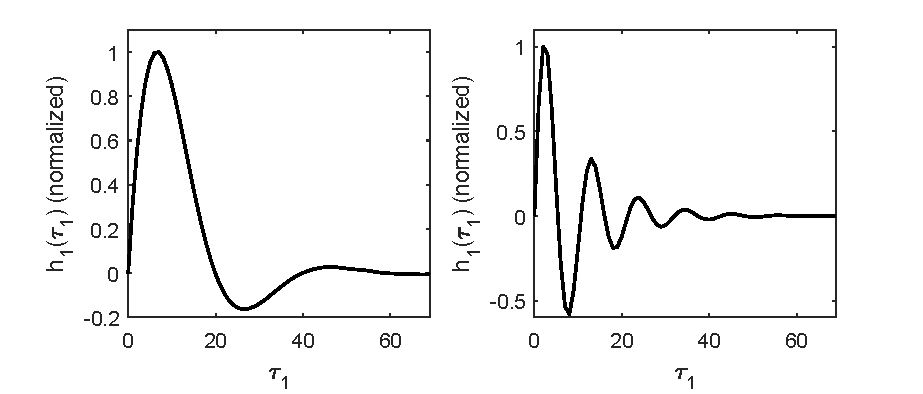
\includegraphics[width = 0.75\textwidth]{Chapter5_RegBFs/Sys2a2b_h1.pdf}
\caption{Normalized impulse response of the linear filter for Sys2a/Sys3/Sys4/Sys5 (left) and Sys2b (right)}
\label{fig:Sys2a2bLinear}
\end{figure}
The corresponding optimal basis function expansions are plotted in Figure \ref{fig:Sys2a2bBF} up to $i_1 = 10$. It is clear for Sys2b that a KBF expansion is the more suitable choice, since the resonant behaviour can be captured in a more compact set of basis functions.
\begin{figure}[!h]
\centering
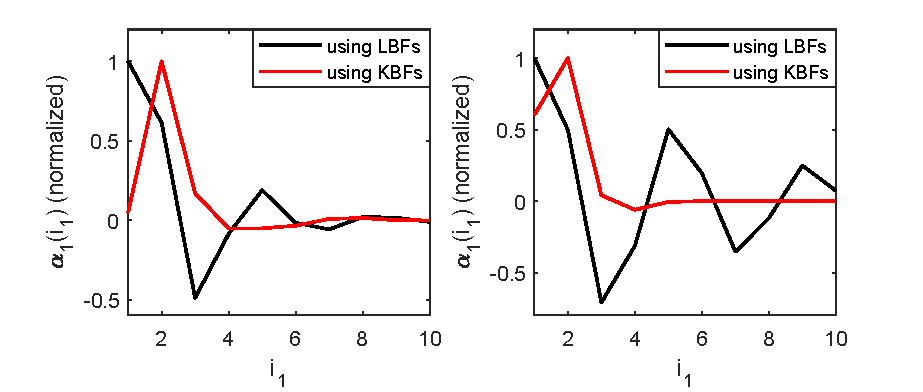
\includegraphics[width = 0.75\textwidth]{Chapter5_RegBFs/Sys2a2b_alpha1.pdf}
\caption{Normalized optimal LBF/KBF expansion coefficients of the linear filter for Sys2a/Sys3/Sys4/Sys5 (left) and Sys2b (right)}
\label{fig:Sys2a2bBF}
\end{figure}

For each system and method, Monte Carlo studies are performed at Signal to Noise Ratios (SNR) of 20dB and 5dB, with 100 realizations per setting. The input, $u$, is constructed as a white Gaussian signal, $u(t) \sim \mathcal{N}(0,1)$, and the data length chosen to be $N=3412$; only 30\% longer than the minimum least squares requirement for Sys2a and Sys2b.

The methods proposed in this chapter are evaluated alongside their unregularized basis function counterparts, as well as a direct time-domain approach. Note that for high nonlinear orders ($M>2$), it is not possible to evaluate the time domain approach due to its immense computational requirements. The details of each method are:

\begin{enumerate}
\item \textbf{ReLS}: The Bayesian regularized method from \cite{Birpoutsoukis2017} in the time domain, using the TC covariance structure in (\ref{KernelPenalty}), (\ref{TCext}) and (\ref{FinalPenalty}), and tuned using MLM. 
\item \textbf{LBF}/\textbf{KBF}: Least squares estimation of LBF/KBF coefficients using (\ref{LSbf}). Optimal basis-generating hyperparameters are assumed to be known a priori (an oracle assumption).
\item \textbf{ReLBF}/\textbf{ReKBF}: Regularized estimation of LBF/KBF kernels using the proposal (\ref{eq:ReBFanalytic}) and the modified EM approach in Algorithm \ref{alg:BFopt} for hyperparameter tuning and pole selection. 
\end{enumerate}

The time domain method is required to estimate each kernel up to a memory length $n_m=70$, while the basis function methods used a length of $\mathcal{B}_m = 10$. For ReLBF/ReKBF, the optimization tasks in Algorithm \ref{alg:BFopt} are performed using MATLAB's $\text{\tt{GlobalSearch}}$ and $\text{\tt{fmincon}}$ functions, and the iterative procedure is terminated when within a 0.5\% convergence tolerance on all hyperparameters. 

For each method and order, Table \ref{tab:ParamNos_OBFS} shows the calculated number of unique kernel parameters to be estimated, $n_p$, and the total number of hyperparameters, $n_h$. From the table, it is clear that for Sys3, Sys4 and Sys5, ReLS requires an unreasonably high number of parameters, and will become too computationally intensive to be feasible. Hence, we consider only LBF and ReLBF methods for these cases. 

\begin{table}[h]
\centering
\caption{Number of parameters ($n_p$) and hyperparameters ($n_h$) for each method and order}
\label{tab:ParamNos_OBFS}
\begin{tabular}{c|c||ccccc}
\multicolumn{2}{r}{Method:}                                                & ReLS & LBF & KBF & ReLBF & ReKBF \\ \hline \hline
\multirow{2}{*}{\begin{tabular}[c]{@{}l@{}}2nd\\ order\end{tabular}} & $n_p$ &2555 &65 &65 &65 &65 \\
                                                                     & $n_h$ &6 &0 &0 &8 &10 \\ \hline
\multirow{2}{*}{\begin{tabular}[c]{@{}l@{}}3rd\\ order\end{tabular}} & $n_p$ &62,195      &285     &285    &285      &285      \\
                                                                     & $n_h$ &10      &0     &0     &13       &16       \\ \hline
\multirow{2}{*}{\begin{tabular}[c]{@{}l@{}}4th\\ order\end{tabular}} & $n_p$ &1,150,625      &1000     &1000    &1000      &1000       \\
                                                                     & $n_h$ &15      &0     &0     &19       &23   \\ \hline   
\multirow{2}{*}{\begin{tabular}[c]{@{}l@{}}5th\\ order\end{tabular}} & $n_p$ &17,259,389      &3002     &3002    &3002      &3002       \\
                                                                     & $n_h$ &21      &0     &0     &26       &31  
\end{tabular}
\end{table}

\subsection{Results}

For each Monte Carlo study, the estimation errors are quantified with the same validation error metric used in \cite{Birpoutsoukis2017}, calculated by applying a validation input of length 50,000 to both the true system and the estimated system and defining `normalized RMS error' as,
\begin{equation}
E_{NRMS} = \frac{\textrm{rms}(y_{val}-y_{mod})}{\textrm{rms}(y_{val})},
\end{equation}
where $y_{val}$ and $y_{mod}$ are the noise-less outputs of the true and estimated system respectively. 

The second order results, presented as boxplots in Figures \ref{Sys2a_Val} and \ref{Sys2b_Val}, show significant improvements in output prediction using ReLBF and ReKBF. The advantage of Kautz functions for resonant systems is clear in the Sys2b (low damping) results, with ReKBF outperforming all other methods. The unregularized estimates do not perform as well, despite being provided with optimal basis functions prior to identification.

\begin{figure}[!h]
\centering
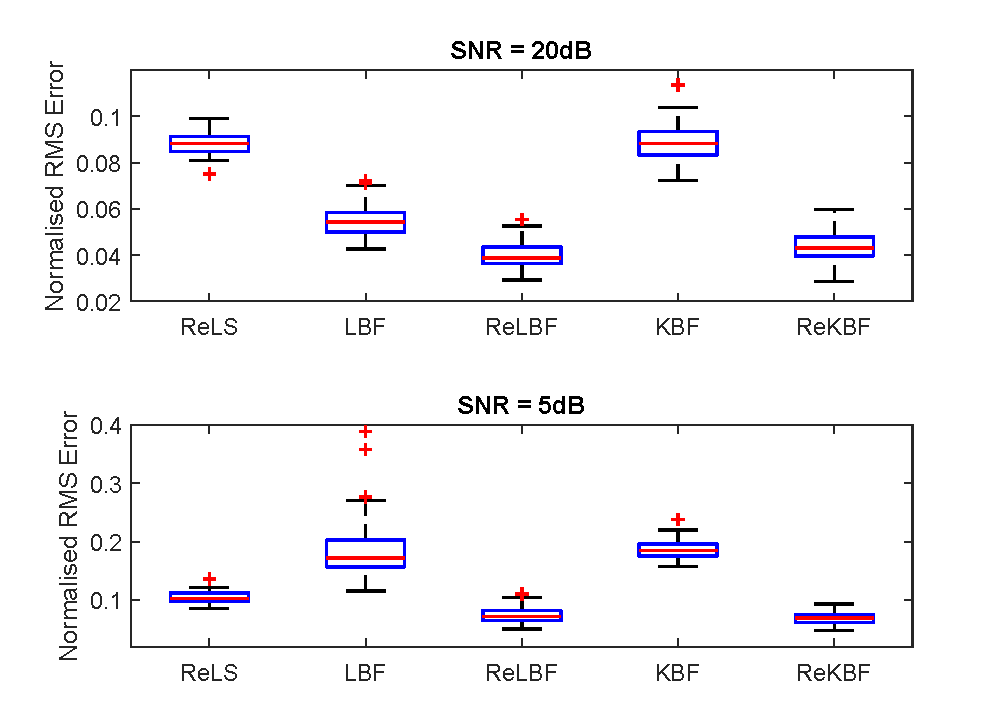
\includegraphics[width = 0.7\textwidth]{Chapter5_RegBFs/Georgios_2ndOrder.pdf}
\caption{Validation errors for Sys2a with SNR = 20dB (top) and 5dB (bottom)}
\label{Sys2a_Val}
\end{figure}

\begin{figure}[!h]
\centering
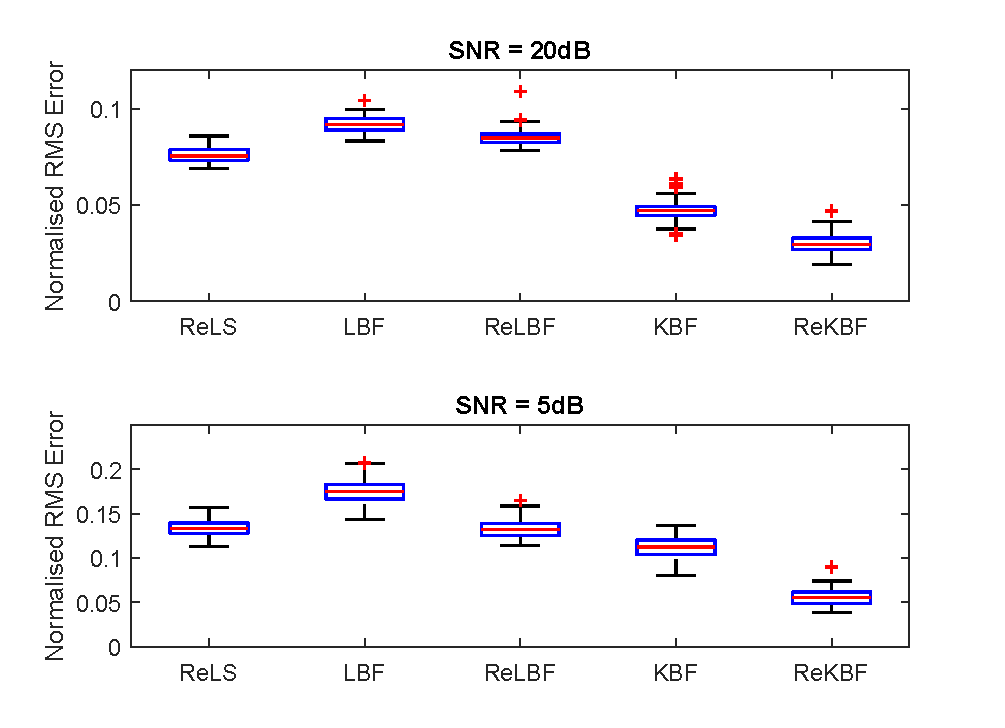
\includegraphics[width = 0.7\textwidth]{Chapter5_RegBFs/Resonant_2ndOrder.pdf}
\caption{Validation errors for Sys2b with SNR = 20dB (top) and 5dB (bottom)}
\label{Sys2b_Val}
\end{figure}

%\begin{table}[t]
%\centering
%\caption{Mean computation times and parameter numbers for 2nd order estimates}
%\label{tab:MeanCompTimes_OBFs}
%\begin{tabular}{c|rrrrr}
%Method & ReLS  & LBF & KBF  & ReLBF & ReKBF \\ \hline
%Time (s) & 375.8 & 0.8 & 1.7 & 37.2  & 53.5 \\
%$n_p$ &2555 &135 &135 &135 &135 \\
%$n_h$ &6 &0 &0 &8 &10
%\end{tabular}
%\end{table}

The validation errors for Sys3, Sys4 and Sys5 are given in Figures \ref{Sys3_Val}, \ref{Sys4_Val} and \ref{Sys5_Val} respectively, which highlight the benefit of the regularized basis function method in lowering model error to tolerable levels. The time domain method, ReLS, requires unreasonably high numbers of parameters and hence is computationally unfeasible. The least squares LBF model estimates, while computationally tractable, produce extremely innacurate predictions. The newly proposed regularized method, however, obtains estimates with reasonable accuracy and computation time using a standard computer architecture, which would not previously have been possible with existing estimation methods under these experimental conditions. For comparison, mean computation times are provided, in Table \ref{tab:MeanCompTimes_OBFs}, for the attempted methods at each order. 

\begin{figure}[!h]
\centering
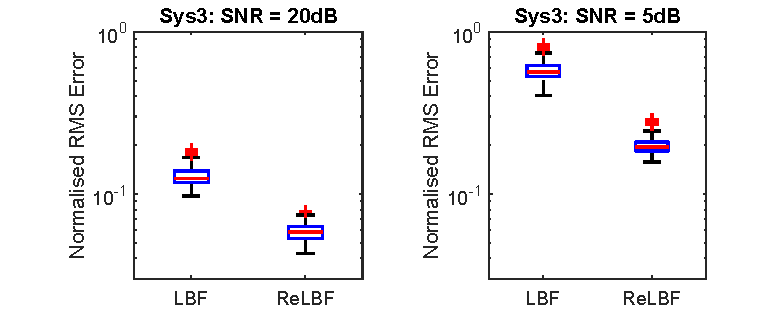
\includegraphics[width = 0.7\textwidth]{Chapter5_RegBFs/Georgios_3rdOrder.pdf}
\caption{Validation errors for Sys3 with SNR = 20dB (left) and 5dB (right)}
\label{Sys3_Val}
\end{figure}
\begin{figure}[!h]
\centering
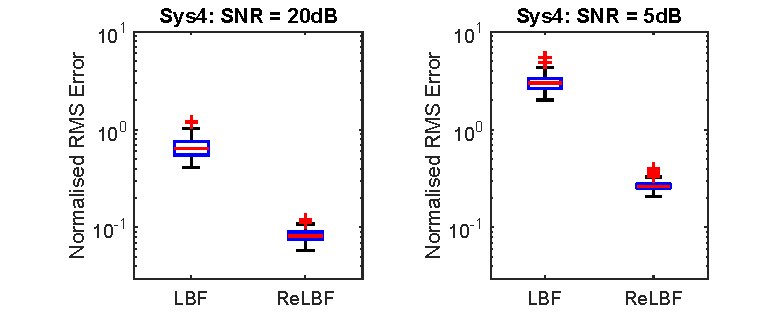
\includegraphics[width = 0.7\textwidth]{Chapter5_RegBFs/Georgios_4thOrder.pdf}
\caption{Validation errors for Sys4 with SNR = 20dB (left) and 5dB (right)}
\label{Sys4_Val}
\end{figure}
\begin{figure}[!h]
\centering
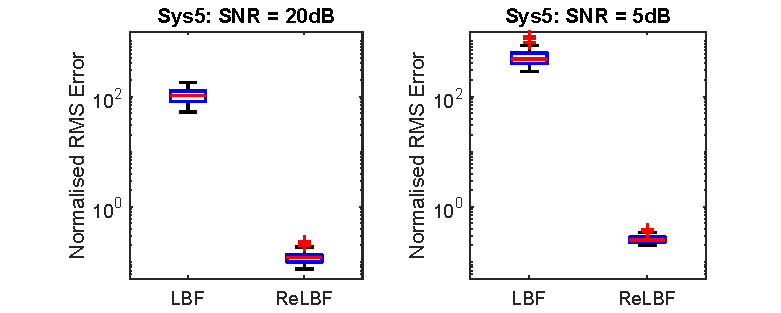
\includegraphics[width = 0.7\textwidth]{Chapter5_RegBFs/Georgios_5thOrder.pdf}
\caption{Validation errors for Sys5 with SNR = 20dB (left) and 5dB (right)}
\label{Sys5_Val}
\end{figure}
\begin{table}[!h]
\centering
\caption{Mean computation time (s) for each method and order}
\label{tab:MeanCompTimes_OBFs}
\begin{tabular}{c||ccccc}
\multicolumn{1}{r}{Method:}                                              & ReLS & LBF & KBF & ReLBF & ReKBF \\ \hline \hline
2nd order	& 376 & 0.4 & 0.9 & 22  & 32 \\
3rd order &-&0.7&-&48&- \\
4th order	&-&1.3&-&228&- \\
5th order	&-&4.3&-&3687&- \\
\end{tabular}
\end{table}

\section{Conclusion}

This chapter makes a novel proposal to combine the techniques of Bayesian regularization and basis function modeling for the purpose of Volterra series estimation. Some theoretical motivation is provided for imposing standard covariance structures on the resultant basis function kernels, and a modified EM algorithm is constructed as an extension of the results in Chapter \ref{chap:4}. The extended algorithm is capable of optimizing both the covariance hyperparameters and the basis-generating hyperparameters, and the iterative procedure will scale more favourably with series order than a direct marginal likelihood approach. The performance of the proposed estimation method has been compared against unregularized least squares estimates, and estimates directly in the time domain, with improved output prediction in all test cases. Furthermore, under the experimental conditions considered in the simulation examples, the proposed method allowed access to computationally feasible and accurate estimates at higher series orders than was previously possible with existing methods in the literature. 

Regularized basis function estimation is clearly a promising tool in addressing the major challenge of time domain Volterra series identification: accuracy and computational feasibility for high order models under arbitrary experimental conditions. 

%There is still work which can be done in this area, for example in exploring the convergence properties of the modified EM Algorithm \ref{alg:BFopt}, which does not become a traditional EM sequence until the basis generating hyperparameters converge. The method can also be extended to other sets of basis functions, particularly those which have already found success in unregularized Volterra series problems.  

\begin{subappendices}
\section{Long division of Laguerre basis function filters}
\label{append:LongDivision}

For a rational transfer function in the $z$-domain, performing a polynomial long division between the numerator and denominator will produce the corresponding impulse response. For example, long division of the transfer function $\frac{1}{z-p}$ for some pole $p \in \mathbb{R}$ will produce
\begin{equation}
0 + 1z^{-1} + p z^{-2} + p^2 z^{-3} + \hdots + p^{i-1} z^{-i} + \hdots,
\end{equation}
where the sequence of coefficients, $[0, 1, p, p^2, \hdots, p^{i-1}, \hdots]$, is the impulse response.

The same process is now applied to the arbitrary order Laguerre filter in (\ref{eq:LongDivResult}), to reveal the structure of the filter's impulse response: 
\begin{sidewaystable}

\small

\begin{alignat*}{9}
&\mathbf{0} &+ &\mathbf{\big[p_{i-1,1}(i) a^{i-1} \big]}z^{-1} &+&\mathbf{\big[p_{i-1,4}(i) a^{i-2}\big]} z^{-2} &+&\mathbf{\big[p_{i-1,8}(i) a^{i-3}\big]} z^{-3} &+ &\hdots \\ \cline{2-10} 
z^i + \sum_{k=0}^{i-1} p_{k,2}(i) a^{i-k} z^k \smash{\Bigg)} &0z^i &+ &\sum_{k=0}^{i-1} p_{k,1}(i) a^k z^k & & & \\
&0 &+ &0 &&&&&&	\tag{end of step 0}\\ \cline{3-10} 
&&  &\sum_{k=0}^{i-1} p_{k,1}(i) a^k z^k &&&&&&  \tag{remove $i-1$ from sum}\\
&&= &p_{i-1,1}(i) a^{i-1} z^{i-1} &+ &\sum_{k=1}^{i-1} p_{k-1,1}(i) a^{k-1} z^{k-1} &&&& \tag{extract $f_i(1)$ and multiply out}\\
&& &p_{i-1,1}(i) a^{i-1} z^{i-1} &+ &\sum_{k=1}^{i-1} p_{k-1,3}(i) a^{2i-k-1} z^{k-1} &+ &\hdots && \tag{end of step 1}\\ \cline{5-10} 
&& & & &\sum_{k=1}^{i-1} (p_{k-1,1}(i) - p_{k-1,3}(i)a^{2i-2k}) a^{k-1} z^{k-1} &+ &\hdots \tag{remove $i-1$ from sum}\\
&&& &= &p_{i-1,4}(i)a^{i-2}z^{i-2} &+ &\sum_{k=2}^{i-1} (p_{k-2,1}(i) - p_{k-2,5}(i)a^{2i-2k}) a^{k-2} z^{k-2} &+ &\hdots \\
&&& & &p_{i-1,4}(i)a^{i-2}z^{i-2} &+ &\sum_{k=2}^{i-1} p_{k-2,6}(i)a^{2i-k-2} z^{k-2} &+ &\hdots \tag{end of step 2}\\ \cline{7-10} 
&&& & & & &\sum_{k=2}^{i-1} (p_{k-2,1}(i)-p_{k-2,7}(i)a^{2i-2k})a^{k-2} z^{k-2} &+ &\hdots \\
&&& & & &= &p_{i-1,8}(i)a^{i-3} z^{i-3} &+ &\sum_{k=3}^{i-1} \hdots \\
&&& & & & &p_{i-1,8}(i)a^{i-3} z^{i-3} &+ &\sum_{k=3}^{i-1} \hdots \\ \cline{9-10}  \\
&&& & & & & \text{and so on up to step $i-1$} 
\end{alignat*}

\normalsize

\end{sidewaystable}

\end{subappendices}
